\section*{Behavior design}
\subsection*{Protocol state machines}
In this section we will explain, on a high abstraction level, what the protocol state machines does.
\subsubsection*{Webserver - Enterprise protocol}
\begin{figure}[H]
\centering
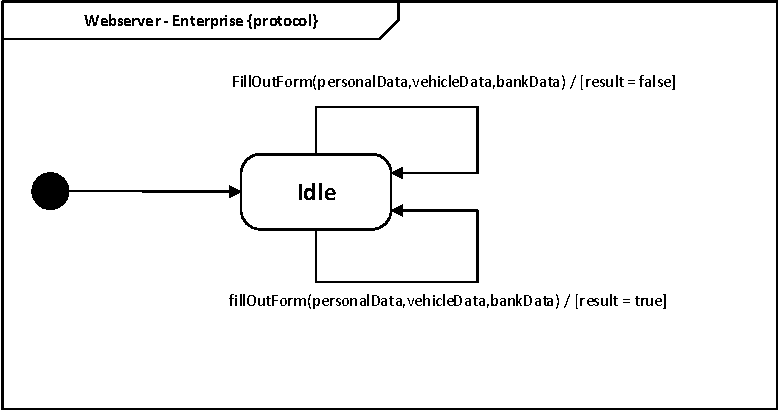
\includegraphics[width=0.7\linewidth]{img/protocol_state_machine/protocol_state_machine_webserver_to_enterprise.png}
\caption{The communication protocol for buying toll tags}
\label{fig:protocol_state_machine_webserver_to_enterprise}
\end{figure}

\subsubsection*{Touchscreen protocol}
\begin{figure}[H]
\centering
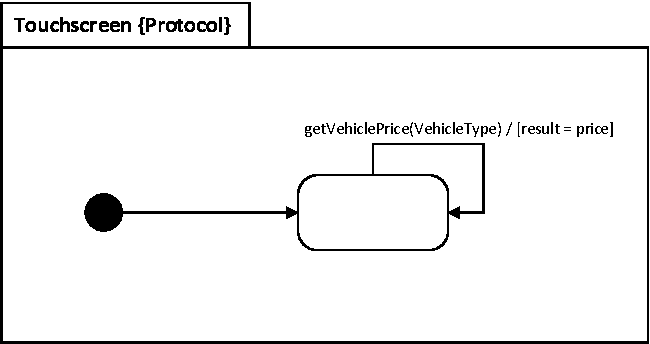
\includegraphics[width=0.7\linewidth]{img/protocol_state_machine/protocol_state_machine_touchscreen.png}
\caption{Protocol statemachine for the touchscreen}
\label{fig:protocol_state_machine_touchscreen}
\end{figure}
The diagram in \autoref{fig:protocol_state_machine_touchscreen} shows the communication protocol for getting the price for different vehicle types. It's used by customers if it is a credit card lane, and the cashier if it is a cash lane.

\subsubsection*{Antenna protocol}
\begin{figure}[H]
\centering
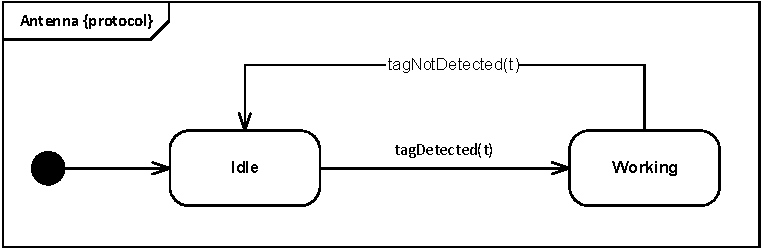
\includegraphics[width=0.7\linewidth]{img/protocol_state_machine/protocol_state_machine_antenna.png}
\caption{The interface the antenna uses, to send out messages when cars are detected}
\label{fig:protocol_state_machine_antenna}
\end{figure}

\subsubsection*{Credit card reader protocol}
\begin{figure}[H]
\centering
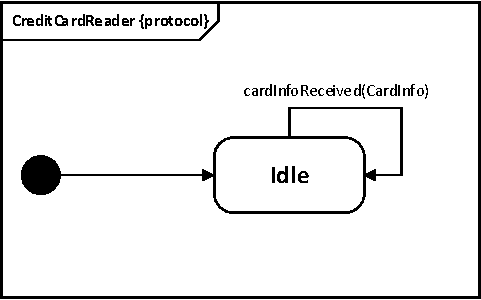
\includegraphics[width=0.7\linewidth]{img/protocol_state_machine/protocol_state_machine_tlc_to_ccr.png}
\caption{The interface for sending data about credit card information}
\label{fig:protocol_state_machine_tlc_to_ccr}
\end{figure}

\subsubsection*{Toll lane - bank protocol}
\begin{figure}[H]
\centering
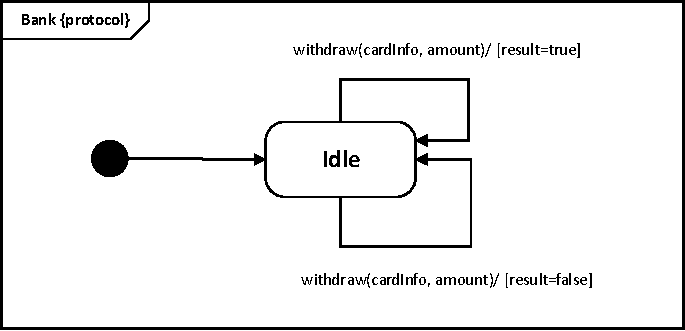
\includegraphics[width=0.7\linewidth]{img/protocol_state_machine/protocol_state_machine_tlc_to_bank.png}
\caption{Communications protocol between the bank and the credit card toll lane is shown}
\label{fig:protocol_state_machine_tlc_to_bank}
\end{figure}

\subsubsection*{Station server - normal toll lane checkout protocol}
\begin{figure}[H]
\centering
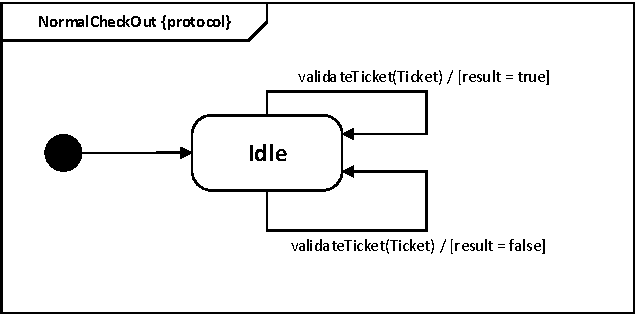
\includegraphics[width=0.7\linewidth]{img/protocol_state_machine/protocol_state_machine_station_server_to_normal_lane_check_out.png}
\caption{Interface to allow toll lanes to validate tickets}
\label{fig:protocol_state_machine_station_server_to_normal_lane_check_out}
\end{figure}

\subsubsection*{Station server - enterprise server protocol}
\begin{figure}[H]
\centering
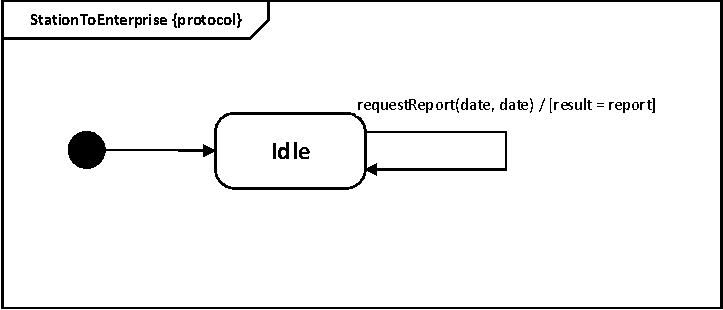
\includegraphics[width=0.7\linewidth]{img/protocol_state_machine/protocol_state_machine_station_server_to_enterprise_server.png}
\caption{Interface to use for getting data for the generation of reports}
\label{fig:protocol_state_machine_station_server_to_enterprise_server}
\end{figure}

\subsubsection*{Express toll lane checkout - station server protocol}
\begin{figure}[H]
\centering
\includegraphics[width=0.7\linewidth]{img/protocol_state_machine/protocol_state_machine_station_server with_toll_computer_check_out.png}
\caption{The communication protocol for checking out toll tag}
\label{fig:protocol_state_machine_station_server with_toll_computer_check_out}
\end{figure}

\subsubsection*{Ticket reader protocol}
\begin{figure}[H]
\centering
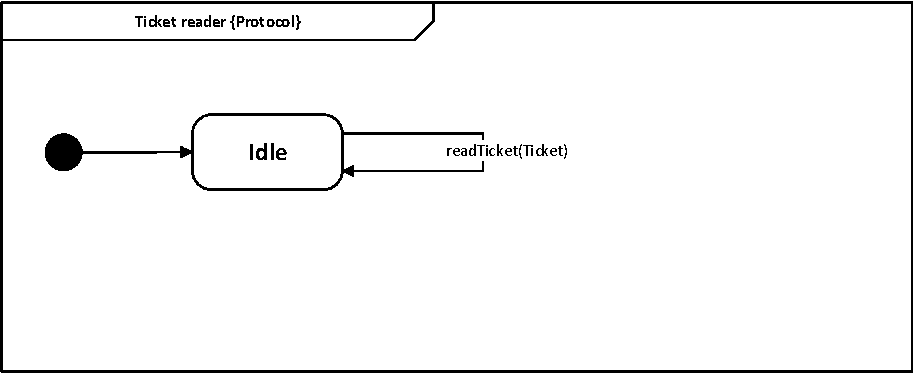
\includegraphics[width=0.7\linewidth]{img/protocol_state_machine/protocol_state_machine_ticket_reader.png}
\caption{The communication protocol for the ticket reader used during checkout for non-tag checkout}
\label{fig:protocol_state_machine_ticket_reader}
\end{figure}

\subsubsection*{Enterprise server - station server protocol}
\begin{figure}[H]
\centering
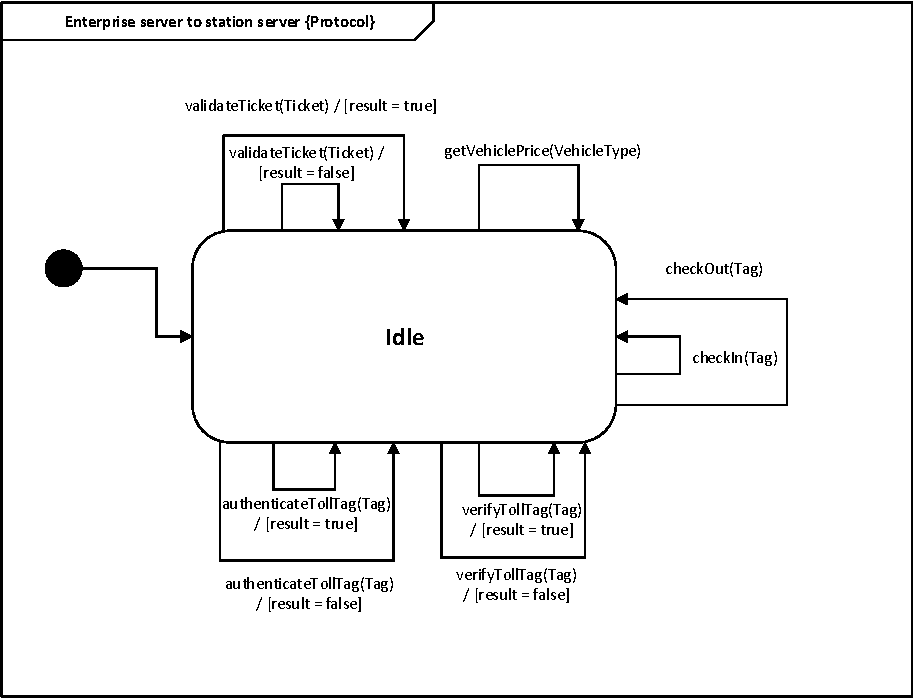
\includegraphics[width=0.7\linewidth]{img/protocol_state_machine/protocol_state_machine_enterprise_server_to_station_server.png}
\caption{The communication protocol between the enterprise server and the station server}
\label{fig:protocol_state_machine_enterprise_server_to_station_server}
\end{figure}

\subsubsection*{Cash register protocol}
\begin{figure}[H]
\centering
\includegraphics[width=0.7\linewidth]{img/protocol_state_machine/protocol_state_machine_CR_TLC.png}
\caption{The communication protocol the cash register offers}
\label{fig:protocol_state_machine_CR_TLC}
\end{figure}

\subsubsection*{Barrier protocol}
\begin{figure}[H]
\centering
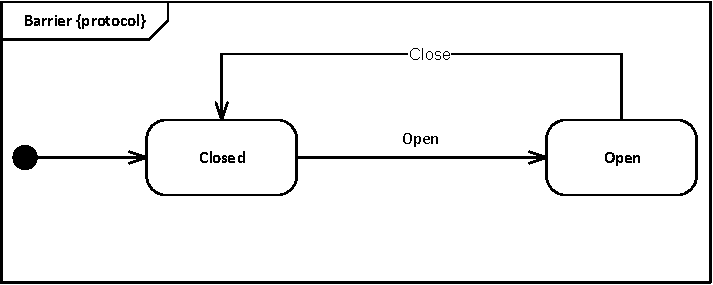
\includegraphics[width=0.7\linewidth]{img/protocol_state_machine/protocol_state_machine_barrier.png}
\caption{The communication protocol the barrier offers}
\label{fig:protocol_state_machine_barrier}
\end{figure}

\subsubsection*{Enterprise client - enterprise server protocol}
\begin{figure}[H]
\centering
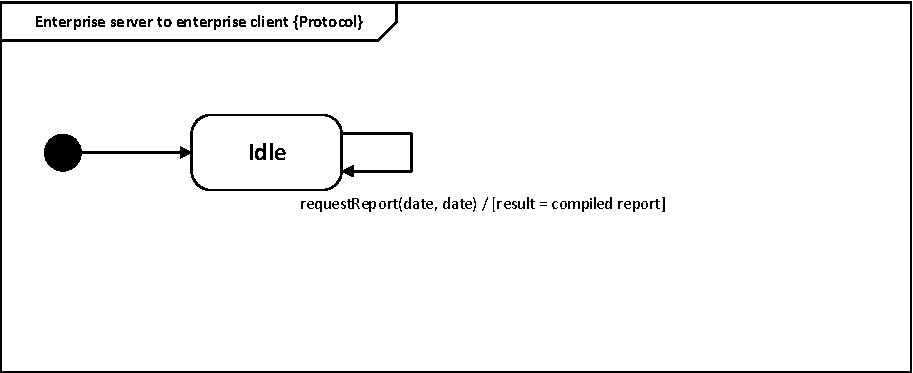
\includegraphics[width=0.7\linewidth]{img/protocol_state_machine/protocol_state_machine_enterprise_server_to_enterprise_client.png}
\caption{The interface that facilitates the requestReport functionality needed for show reports between enterprise client and server}
\label{fig:protocol_state_machine_enterprise_server_to_enterprise_client}
\end{figure}

\subsubsection*{Enterprise manager - enterprise client protocol}
\begin{figure}[H]
\centering
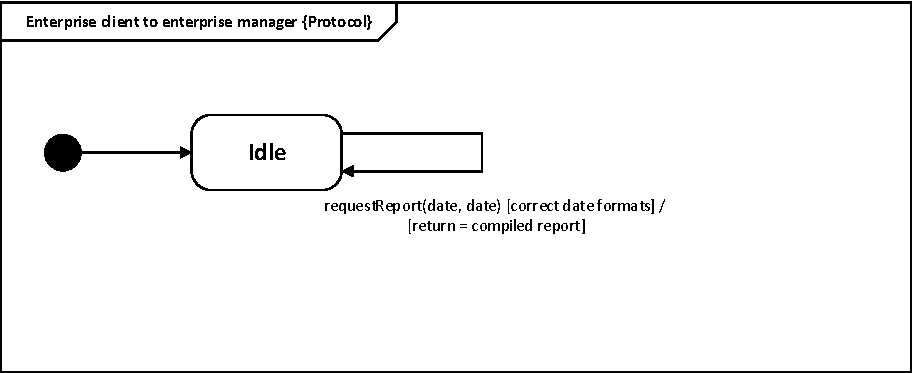
\includegraphics[width=0.7\linewidth]{img/protocol_state_machine/protocol_state_machine_enterprise_client_enterprise_manager.png}
\caption{The interface the enterprise client provides to the enterprise manager}
\label{fig:protocol_state_machine_enterprise_client_enterprise_manager}
\end{figure}